\documentclass[a4paper, 14pt]{extarticle}

% Поля
%--------------------------------------
\usepackage{geometry}
\geometry{a4paper,tmargin=2cm,bmargin=2cm,lmargin=3cm,rmargin=1cm}
%--------------------------------------


%Russian-specific packages
%--------------------------------------
\usepackage[T2A]{fontenc}
\usepackage[utf8]{inputenc} 
\usepackage[english, main=russian]{babel}
%--------------------------------------

\usepackage{textcomp}

% Красная строка
%--------------------------------------
\usepackage{indentfirst}               
%--------------------------------------             


%Graphics
%--------------------------------------
\usepackage{graphicx}
\graphicspath{ {./images/} }
\usepackage{wrapfig}
%--------------------------------------

% Полуторный интервал
%--------------------------------------
\linespread{1.3}                    
%--------------------------------------

%Выравнивание и переносы
%--------------------------------------
% Избавляемся от переполнений
\sloppy
% Запрещаем разрыв страницы после первой строки абзаца
\clubpenalty=10000
% Запрещаем разрыв страницы после последней строки абзаца
\widowpenalty=10000
%--------------------------------------

%Списки
\usepackage{enumitem}

%Подписи
\usepackage{caption} 

%Гиперссылки
\usepackage{hyperref}

\hypersetup {
	unicode=true
}

%Рисунки
%--------------------------------------
\DeclareCaptionLabelSeparator*{emdash}{~--- }
\captionsetup[figure]{labelsep=emdash,font=onehalfspacing,position=bottom}
%--------------------------------------

\usepackage{tempora}

%Листинги
%--------------------------------------
\usepackage{listings}
\lstset{
  basicstyle=\ttfamily\footnotesize, 
  %basicstyle=\footnotesize\AnkaCoder,        % the size of the fonts that are used for the code
  breakatwhitespace=false,         % sets if automatic breaks shoulbd only happen at whitespace
  breaklines=true,                 % sets automatic line breaking
  captionpos=t,                    % sets the caption-position to bottom
  inputencoding=utf8,
  frame=single,                    % adds a frame around the code
  keepspaces=true,                 % keeps spaces in text, useful for keeping indentation of code (possibly needs columns=flexible)
  keywordstyle=\bf,       % keyword style
  numbers=left,                    % where to put the line-numbers; possible values are (none, left, right)
  numbersep=5pt,                   % how far the line-numbers are from the code
  xleftmargin=25pt,
  xrightmargin=25pt,
  showspaces=false,                % show spaces everywhere adding particular underscores; it overrides 'showstringspaces'
  showstringspaces=false,          % underline spaces within strings only
  showtabs=false,                  % show tabs within strings adding particular underscores
  stepnumber=1,                    % the step between two line-numbers. If it's 1, each line will be numbered
  tabsize=2,                       % sets default tabsize to 8 spaces
  title=\lstname                   % show the filename of files included with \lstinputlisting; also try caption instead of title
}
%--------------------------------------

%%% Математические пакеты %%%
%--------------------------------------
\usepackage{amsthm,amsfonts,amsmath,amssymb,amscd}  % Математические дополнения от AMS
\usepackage{mathtools}                              % Добавляет окружение multlined
\usepackage[perpage]{footmisc}
%--------------------------------------

%--------------------------------------
%			НАЧАЛО ДОКУМЕНТА
%--------------------------------------

\begin{document}

%--------------------------------------
%			ТИТУЛЬНЫЙ ЛИСТ
%--------------------------------------
\begin{titlepage}
\thispagestyle{empty}
\newpage


%Шапка титульного листа
%--------------------------------------
\vspace*{-60pt}
\hspace{-65pt}
\begin{minipage}{0.3\textwidth}
\hspace*{-20pt}\centering

\includegraphics[width=\textwidth]{emblem}
\end{minipage}
\begin{minipage}{0.67\textwidth}\small \textbf{
\vspace*{-0.7ex}
\hspace*{-6pt}\centerline{Министерство науки и высшего образования Российской Федерации}
\vspace*{-0.7ex}
\centerline{Федеральное государственное бюджетное образовательное учреждение }
\vspace*{-0.7ex}
\centerline{высшего образования}
\vspace*{-0.7ex}
\centerline{<<Московский государственный технический университет}
\vspace*{-0.7ex}
\centerline{имени Н.Э. Баумана}
\vspace*{-0.7ex}
\centerline{(национальный исследовательский университет)>>}
\vspace*{-0.7ex}
\centerline{(МГТУ им. Н.Э. Баумана)}}
\end{minipage}
%--------------------------------------

%Полосы
%--------------------------------------
\vspace{-25pt}
\hspace{-35pt}\rule{\textwidth}{2.3pt}

\vspace*{-20.3pt}
\hspace{-35pt}\rule{\textwidth}{0.4pt}
%--------------------------------------

\vspace{1.5ex}
\hspace{-35pt} \noindent \small ФАКУЛЬТЕТ\hspace{80pt} <<Информатика и системы управления>>

\vspace*{-16pt}
\hspace{47pt}\rule{0.83\textwidth}{0.4pt}

\vspace{0.5ex}
\hspace{-35pt} \noindent \small КАФЕДРА\hspace{50pt} <<Теоретическая информатика и компьютерные технологии>>

\vspace*{-16pt}
\hspace{30pt}\rule{0.866\textwidth}{0.4pt}
  
\vspace{11em}

\begin{center}
\Large {\bf Лабораторная работа № 1} \\
\large {\bf по курсу <<Разработка мобильных приложений>>} \\
\large <<Графический пользовательский интерфейс в Dart>>
\end{center}\normalsize

\vspace{8em}


\begin{flushright}
  {Студентка группы ИУ9-72Б Самохвалова П. С. \hspace*{15pt}\\
  \vspace{2ex}
  Преподаватель Посевин Д. П.\hspace*{15pt}}
\end{flushright}

\bigskip

\vfill
 

\begin{center}
\textsl{Москва 2023}
\end{center}
\end{titlepage}
%--------------------------------------
%		КОНЕЦ ТИТУЛЬНОГО ЛИСТА
%--------------------------------------

\renewcommand{\ttdefault}{pcr}

\setlength{\tabcolsep}{3pt}
\newpage
\setcounter{page}{2}

\section{Цель работы}\label{Sect::goal}

Научиться создавать приложения с графическим пользовательским интерфейсом c использованием фреймворка Flutter на языке программирования Dart.

\section{Задание}\label{Sect::task}

В течение лабораторной работы нужно разработать программу, рисующую на экране
мобильного устройства одно из изображений, перечисленных в таблице ниже. Программа
должна иметь графический пользовательский интерфейс, через который пользователь может
задавать параметры изображения. Изображение должно перерисовываться автоматически при
изменении любого параметра. Значения параметров, обозначенных в таблице латинскими
буквами, представляют собой неотрицательные целые числа. Когда в описании изображения
говорится о выборе цвета, подразумевается выбор из нескольких предопределённых
альтернатив (например, красный, зелёный или синий).

Индивидуальный вариант:

Прямоугольный треугольник выбранного цвета с катетами a и b, вписанный в окружность.

\section{Практическая реализация}\label{Sect::code}

Исходный код программы представлен в листинге~\ref{lst:code1}.

\begin{lstlisting}[language={},caption={Графический пользовательский интерфейс в Dart},label={lst:code1}]
import 'dart:ui';
import 'package:flutter/material.dart';
import 'dart:math' as math;

void main() => runApp(MyApp());

class MyApp extends StatelessWidget {
  @override
  Widget build(BuildContext context) {
    return MaterialApp(
      title: 'Flutter Custom Painter',
      theme: ThemeData(
        primarySwatch: Colors.blue,
      ),
      home: MyPainter(),
    );
  }
}

class MyPainter extends StatefulWidget {
  @override
  _MyPainterState createState() => _MyPainterState();
}

class _MyPainterState extends State<MyPainter> {
  var _catetA = 100.0;
  var _catetB = 100.0;
  Color selectedColor = Colors.teal;

  @override
  Widget build(BuildContext context) {
    return Scaffold(
      appBar: AppBar(
        title: Text('Triangle'),
      ),
      body: SafeArea(
        child: Column(
          crossAxisAlignment: CrossAxisAlignment.start,
          children: <Widget>[
            RadioListTile(
              title: Text('Red'),
              value: Colors.red,
              groupValue: selectedColor,
              onChanged: (value) {
                setState(() {
                  selectedColor = value!;
                });
              },
            ),
            RadioListTile(
              title: Text('Yellow'),
              value: Colors.yellow, //unique value
              groupValue: selectedColor ,
              onChanged: (value) {
                setState(() {
                  selectedColor = value!;
                });
              },
            ),
            RadioListTile(
              title: Text('Green'),
              value: Colors.green,
              groupValue: selectedColor,
              onChanged: (value) {
                setState(() {
                  selectedColor = value!;
                });
              },
            ),

            Expanded(
              child: CustomPaint(
                painter: ShapePainter(_catetA, _catetB, selectedColor),
                child: Container(),
              ),
            ),

            Padding(
              padding: const EdgeInsets.only(left: 16.0),
              child: Text('Cathet A'),
            ),
            Slider(
              value: _catetA,
              min: - MediaQuery.of(context).size.height / 2,
              max: MediaQuery.of(context).size.height / 2,
              onChanged: (value) {
                setState(() {
                  _catetA = value;
                });
              },
            ),

            Padding(
              padding: const EdgeInsets.only(left: 16.0),
              child: Text('Cathet B'),
            ),
            Slider(
              value: _catetB,
              min: - MediaQuery.of(context).size.width / 2,
              max: MediaQuery.of(context).size.width / 2,
              onChanged: (value) {
                setState(() {
                  _catetB = value;
                });
              },
            ),

          ],
        ),
      ),
    );
  }
}

// FOR PAINTING POLYGONS
class ShapePainter extends CustomPainter {

  final double catetA;
  final double catetB;
  final Color shapeColor;
  ShapePainter(this.catetA, this.catetB, this.shapeColor);

  @override
  void paint(Canvas canvas, Size size) {
    var paint = Paint()
      ..color = shapeColor
      ..strokeWidth = 5
      ..strokeCap = StrokeCap.round
      ..style = PaintingStyle.stroke;

    var catA = catetA;
    var catB = catetB;
    var hypo = math.sqrt(math.pow(catA, 2) + math.pow(catB, 2));
    var rad = hypo / 2 ;

    var startAX = size.width / 2;
    var startAY = size.height / 2;
    Offset startA = Offset(startAX , startAY);
    var endAX = size.width / 2;
    var endAY = size.height / 2 - catA;
    Offset endA = Offset(endAX, endAY);
    canvas.drawLine(startA, endA, paint);

    var startBX = size.width / 2;
    var startBY = size.height / 2;
    Offset startB = Offset(startBX , startBY);
    var endBX = size.width / 2 + catB;
    var endBY = size.height / 2;
    Offset endB = Offset(endBX, endBY);
    canvas.drawLine(startB, endB, paint);

    canvas.drawLine(endA, endB, paint);

    Offset center = Offset((endAX + endBX) / 2, (endAY + endBY) / 2);
    canvas.drawCircle(center, rad, paint);

  }

  @override
  bool shouldRepaint(CustomPainter oldDelegate) {
    return false;
  }
}

\end{lstlisting}

\section{Результаты}\label{Sect::res}

Результаты работы программы представлены на рисунках~\ref{fig:img1}~--~\ref{fig:img5}. 

\begin{figure}[!htb]
	\centering
	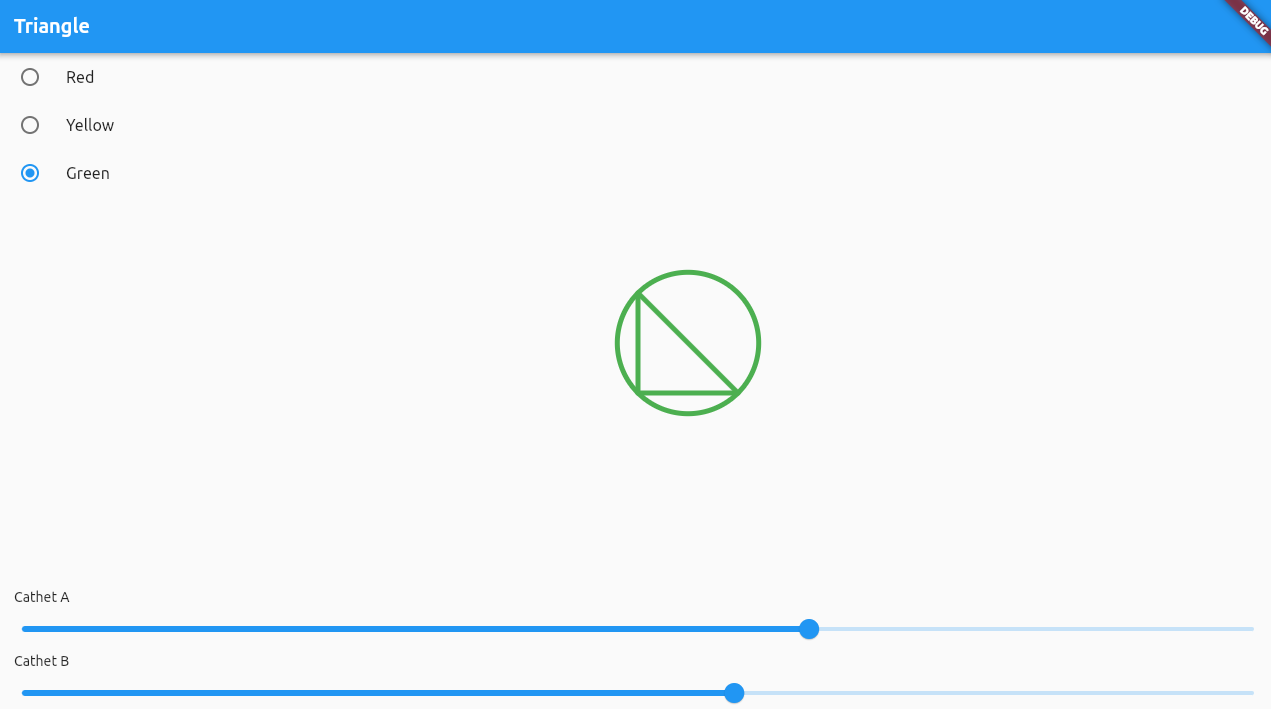
\includegraphics[width=0.8\textwidth]{img1}
\caption{Интерфейс приложения}
\label{fig:img1}
\end{figure}

\begin{figure}[!htb]
	\centering
	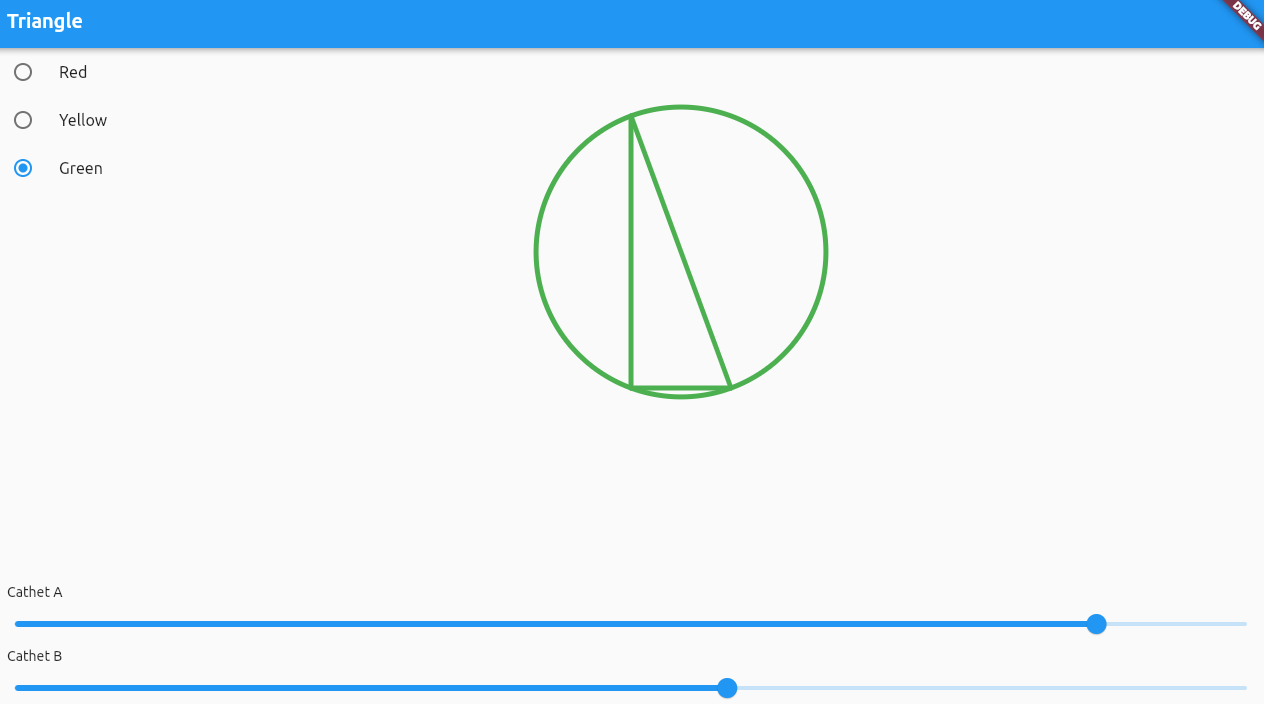
\includegraphics[width=0.8\textwidth]{img2}
\caption{Изменение длины катета}
\label{fig:img2}
\end{figure}

\begin{figure}[!htb]
	\centering
	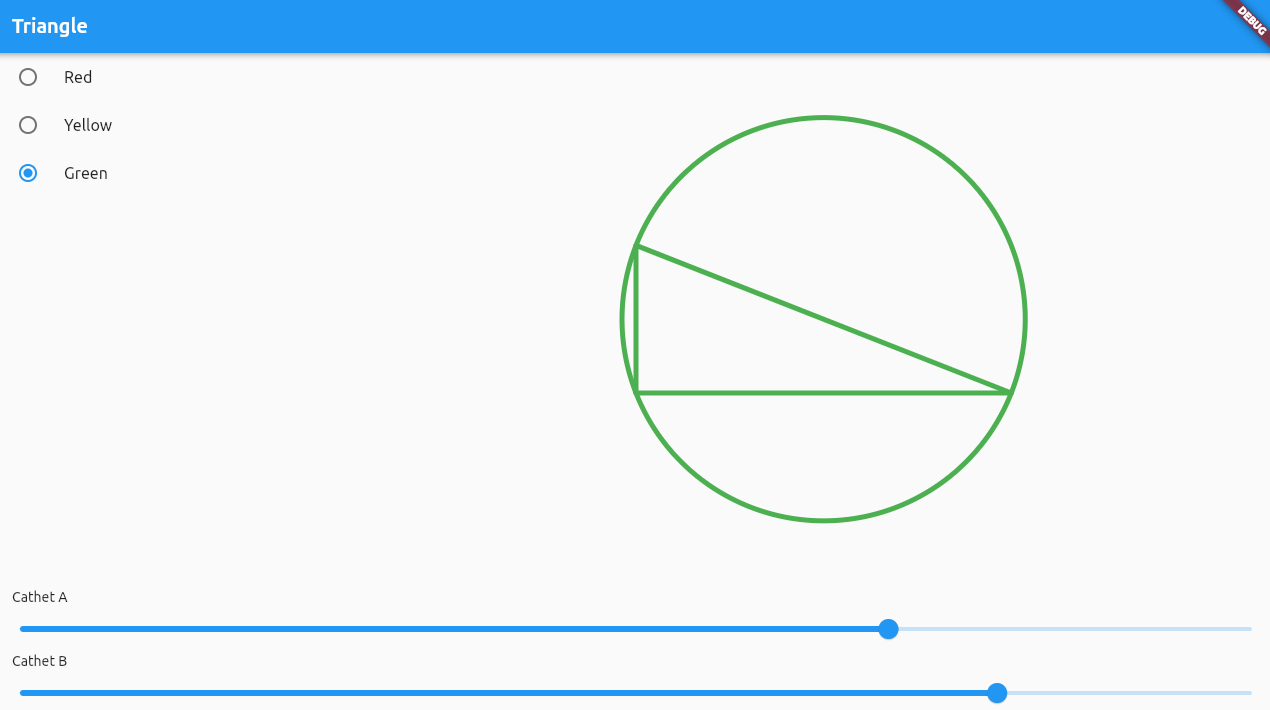
\includegraphics[width=0.8\textwidth]{img3}
\caption{Изменение длины катета}
\label{fig:img3}
\end{figure}

\begin{figure}[!htb]
	\centering
	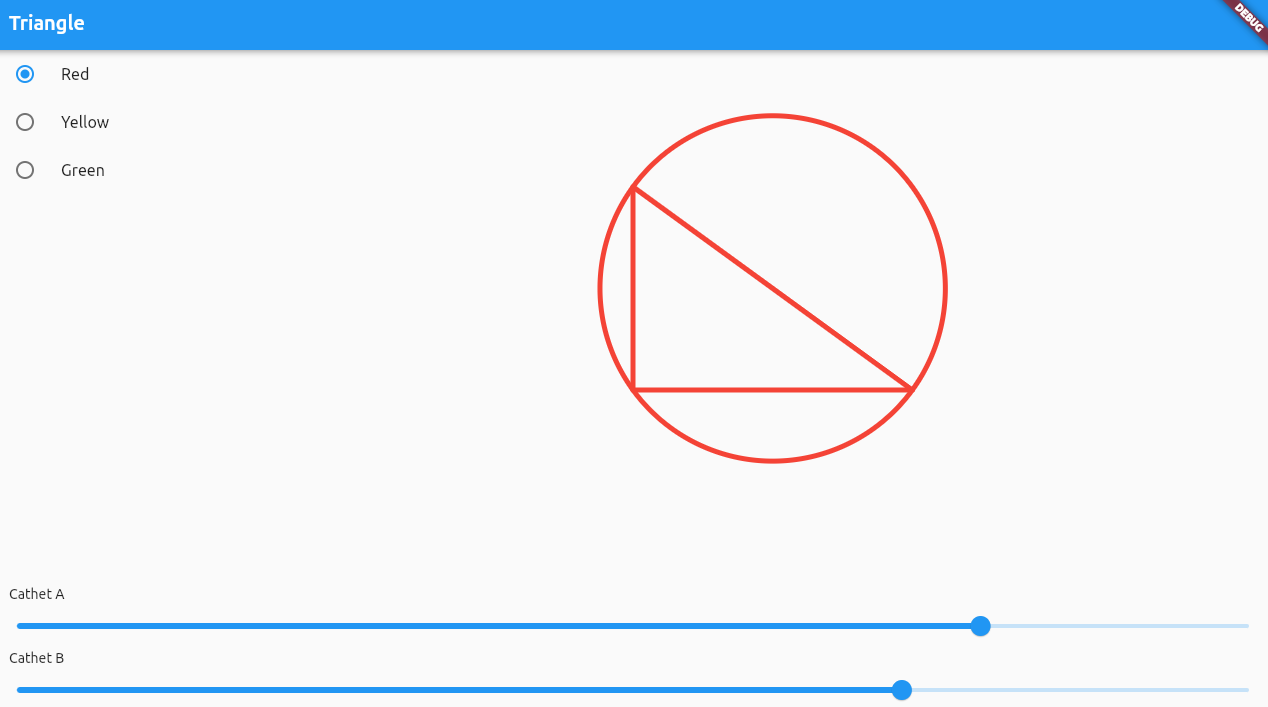
\includegraphics[width=0.8\textwidth]{img4}
\caption{Изменение цвета}
\label{fig:img4}
\end{figure}

\begin{figure}[!htb]
	\centering
	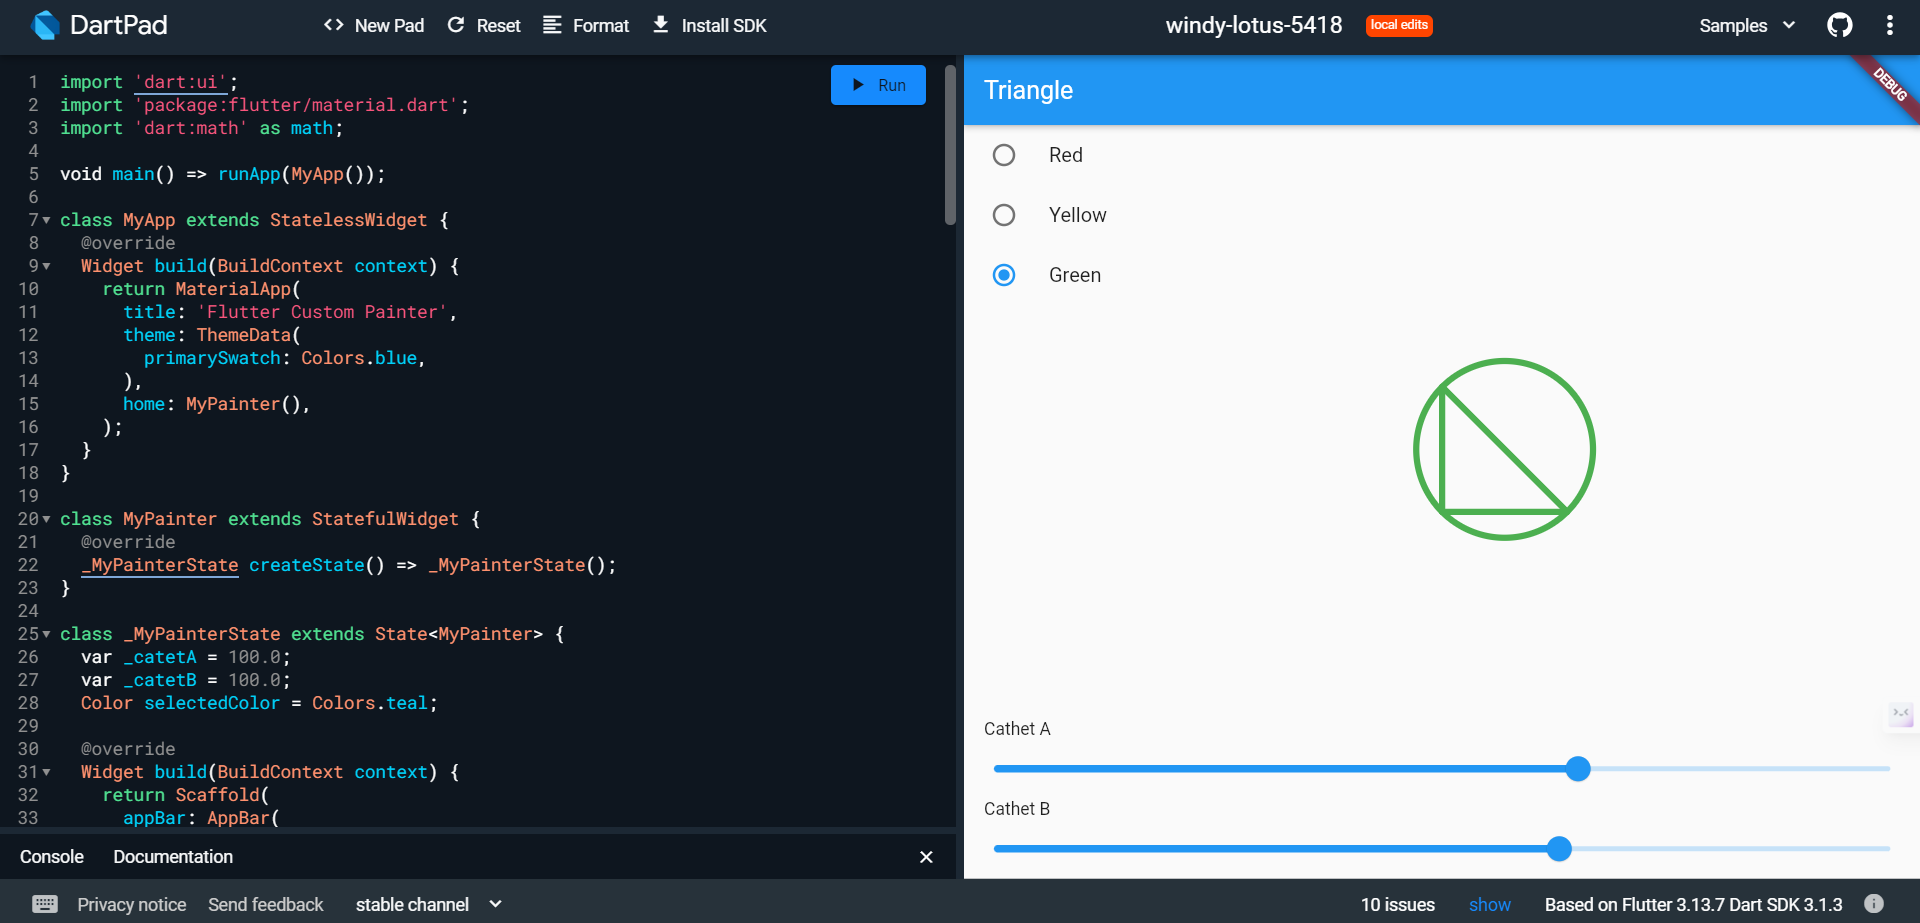
\includegraphics[width=0.8\textwidth]{img5}
\caption{Результат в DartPad}
\label{fig:img5}
\end{figure}

Ссылка на DartPad: 

https://dartpad.dev/?id=560f204e649dac497f0a50255914808e

\section{Выводы}\label{Sect::conclusion}

В результате выполнения лабораторной работы было создано приложения с графическим пользовательским интерфейсом c использованием фреймворка Flutter на языке программирования Dart.

\end{document}
